In Shiny, you express server logic using reactive programming.

The main idea of ​​reactive programming is to specify the dependency graph so that when an input is changed, all related outputs are also updated, for example, we don't need to tell an output to update because due to reactivity, the information is always updated. automatic, making the flow of an application considerably simpler.
  
Reactivity is what makes Shiny applications responsive. Allows the application to update itself instantly whenever the user interacts with the application, requesting any visualization, with updated data.

So the reactive works as it is a way to control which parts of the app are updated, avoiding unnecessary calculations that can slow down your app.
In our app we use reactive functions, as it is a way to control which parts of the app are updated, avoiding unnecessary calculations that can slow down your app.

In our application we use reactive functions as it is a way to control which parts of the application are updated, avoiding unnecessary calculations that can make your application slow.



\begin{figure}[h]
\centering % para centralizarmos a figura
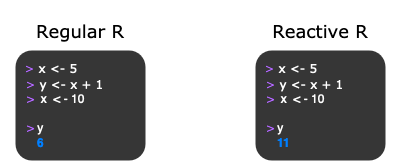
\includegraphics[width=7cm]{images/react.png} 

\caption{Example of Regular R - Reactive R}
\label{figura:qualquernome}
\end{figure}




For example, in our app //PUT AN EXAMPLE OF OUR APP
